\section{2D example}\label{d-example}

A working example of a 2D problem can be found at
\url{https://github.com/cpgr/numbat/blob/master/examples/2D/isotropic/2Dddc.i}.

\subsection{Input file}\label{input-file}

The complete input file for this problem is

\section{Density-driven convective
mixing}\label{density-driven-convective-mixing}

\begin{verbatim}
[Mesh]
  type = GeneratedMesh
  dim = 2
  xmax = 1000
  ymin = -200
  ymax = 0
  nx = 80
  ny = 20
  bias_y = 0.7
[]

[Adaptivity]
  marker = errormarker
  max_h_level = 1
  initial_marker = errormarker
  initial_steps = 1
  [./Indicators]
    [./gradjumpindicator]
      type = GradientJumpIndicator
      variable = concentration
    [../]
  [../]
  [./Markers]
    [./errormarker]
      type = ErrorToleranceMarker
      refine = 0.005
      indicator = gradjumpindicator
    [../]
  [../]
[]

[Variables]
  [./concentration]
    order = FIRST
    family = LAGRANGE
    [./InitialCondition]
      type = PerturbationIC
      variable = concentration
      amplitude = 0.1
      seed = 1
    [../]
  [../]
  [./streamfunction]
    order = FIRST
    family = LAGRANGE
    initial_condition = 0.0
  [../]
[]

[Kernels]
  [./TwoDDarcyDDC]
    type = DarcyDDC
    variable = streamfunction
    concentration_variable = concentration
  [../]
  [./TwoDConvectionDiffusionDDC]
    type = ConvectionDiffusionDDC
    variable = concentration
    streamfunction_variable = streamfunction
  [../]
  [./TimeDerivative]
    type = TimeDerivative
    variable = concentration
  [../]
[]

[AuxVariables]
  [./u]
    order = CONSTANT
    family = MONOMIAL
  [../]
  [./w]
    order = CONSTANT
    family = MONOMIAL
  [../]
[]

[AuxKernels]
  [./uAux]
    type = VelocityDDCAux
    variable = u
    component = x
    streamfunction_variable = streamfunction
  [../]
  [./wAux]
    type = VelocityDDCAux
    variable = w
    component = y
    streamfunction_variable = streamfunction
  [../]
[]

[BCs]
  [./conctop]
    type = DirichletBC
    variable = concentration
    boundary = top
    value = 1.0
  [../]
  [./streamfuntop]
    type = DirichletBC
    variable = streamfunction
    boundary = top
    value = 0.0
  [../]
  [./streamfunbottom]
    type = DirichletBC
    variable = streamfunction
    boundary = bottom
    value = 0.0
  [../]
  [./Periodic]
    [./x]
      variable = 'concentration streamfunction'
      auto_direction = x
    [../]
  [../]
[]

[Executioner]
  type = Transient
  dtmax = 100
  end_time = 4000
  start_time = 1
  solve_type = PJFNK
  nl_abs_tol = 1e-10
  [./TimeStepper]
    type = IterationAdaptiveDT
    dt = 1
    cutback_factor = 0.5
    growth_factor = 2
  [../]
  [./TimeIntegrator]
    type = LStableDirk2
  [../]
[]

[Postprocessors]
  [./boundaryfluxint]
    type = SideFluxIntegral
    variable = concentration
    boundary = top
    diffusivity = 1
  [../]
  [./numdofs]
    type = NumDOFs
  [../]
[]

[Preconditioning]
  [./smp]
    type = SMP
    full = true
    petsc_options = -snes_ksp_ew
    petsc_options_iname = '-pc_type -pc_asm_overlap -sub_pc_type'
    petsc_options_value = 'asm 4 lu'
  [../]
[]

[Outputs]
  [./console]
    type = Console
    perf_log = true
    output_nonlinear = true
  [../]
  [./exodus]
    type = Exodus
    file_base = 2Dddc
    execute_on = 'INITIAL TIMESTEP_END'
  [../]
  [./csvoutput]
    type = CSV
    file_base = 2Dddc
    execute_on = 'INITIAL TIMESTEP_END'
  [../]
[]
\end{verbatim}

\subsection{Running the example}\label{running-the-example}

This example can be run on the commandline using

\begin{verbatim}
numbat-opt -i 2Dddc.i
\end{verbatim}

Alternatively, this file can be run using the \emph{Peacock} gui
provided by MOOSE using

\begin{verbatim}
peacock -i 2Dddc.i
\end{verbatim}

in the directory where \emph{2Dddc.i} resides.

\subsection{Results}\label{results}

This 2D example should take only a few minutes to run to completion,
producing a concentration profile similar to that presented in Figure
\ref{fig:2D}, where several downwelling plumes of high concentration can
be observed:

\begin{figure}[htbp]
\centering
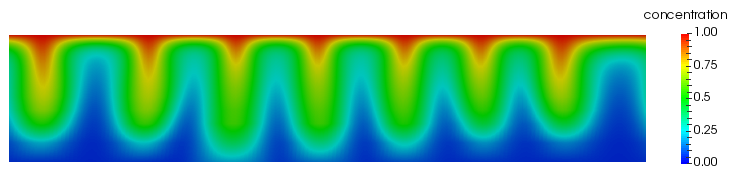
\includegraphics{images/2D.png}
\caption{2D concentration profile\label{fig:2D}}
\end{figure}

 Note that due to the random perturbation applied to the initial
concentration profile, the geometry of the concentration profile
obtained will differ from run to run.

The flux over the top boundary is of particular interest in many cases
(especially convective mixing of \(\textrm{CO}_2\)). This is calculated
in this example file using the \emph{boundaryfluxint} postprocessor in
the input file, and presented in Figure \ref{fig:2Dflux}.

\begin{figure}[htbp]
\centering
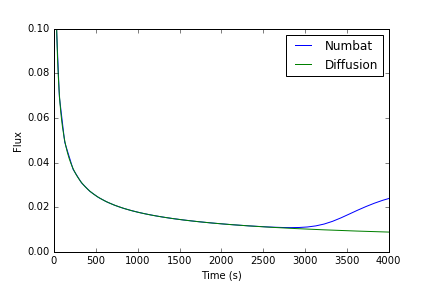
\includegraphics{images/2Dflux.png}
\caption{2D flux across the top boundary\label{fig:2Dflux}}
\end{figure}

 Initially, the flux is purely diffusive, and scales as
\(1 / \sqrt(\pi t)\), where \(t\) is time (shown as the dashed green
line). After some time, the convective instability becomes sufficiently
strong, at which point the flux across the top boundary rapidly
increases (at a time of approximately 1,500 seconds).
